\documentclass[12pt]{article}
\usepackage[utf8]{inputenc}
\usepackage{amsfonts}
\usepackage{amsmath}
\usepackage{graphicx}
\usepackage{fullpage}
\usepackage{subcaption}
\usepackage{float}

\title{Projet COMPLEX\\Problème du VERTEX COVER}
\author{Esther CHOI (3800370)\\Folco BERTINI\\M1 DAC - Groupe 1}

\begin{document}

\maketitle
\tableofcontents

\begin{abstract}
    Ce document constitue le rapport du projet de l'UE COMPLEX, suivie au premier semestre du M1 Informatique à Sorbonne Université. \\
    Les études de performance ont été réalisés avec un processeur Intel \copyright Core \texttrademark i7-8550U 1.80GHz. \\
\end{abstract}

\newpage

\section{Définition du problème}

    Une couverture d'un graphe est un ensemble de sommets qui couvre tous les sommets du graphe. \\
    Le problème \textsc{vertex cover} est défini de la façon suivante :

    \begin{itemize}
        \item entrée : un graphe non orienté G
        \item sortie : une couverture de G de taille minimale
    \end{itemize}

    Le but de ce projet est d'implémenter des algorithmes approchés et exacts pour résoudre le problème \textsc{vertex cover}.

\section{Méthodes approchées}

    \paragraph{1)}
        Soit le graphe $I$ suivant :

        \begin{figure}[h]
            \caption{Graphe $I$}
            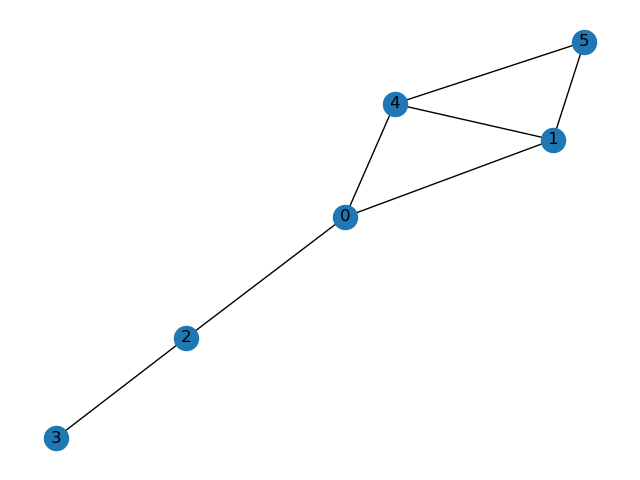
\includegraphics[scale=0.7]{figures/q3-1.png}
            \centering
        \end{figure}

        Une couverture optimale est $C_{opt} = \{0,2,6\}$. L'algorithme glouton renvoie la solution $C = \{0,1,2,5\}$ qui a un sommet de plus (l'exécution complète est donnée en annexe). Ceci montre que algo\_glouton n'est pas optimal et qu'il n'est pas 1.2-approché. \\
        En effet, s'il l'était, alors pour toute instance de \textsc{vertex cover}, le rapport d'approximation entre la solution retournée et une solution optimale serait inférieur ou égal à 1.2. \\
        Or pour l'instance $I$ précédente, ce rapport vaut $r = \frac{|C|}{|C_{opt}|} = \frac{4}{3} \approx 1.33 > 1.2$. \\
        Donc algo\_glouton n'est pas 1.2-approché.

    \paragraph{2)} Comparons les deux algorithmes algo\_couplage et algo\_glouton. \\
        Pour cela, nous avons commencé par calculer $N_{max}$ comme suggéré dans l'énoncé. Nous avons pris $p = 1$ et nous nous sommes limités à un temps d'éxécution de 10 secondes. Nous avons ainsi trouvé $N_{max} = 600$.

        \begin{enumerate}
            \item \textit{Comparaison du point de vue du temps de calcul} : \\
            Les graphiques suivants montrent les temps de calcul pris par les deux algorithmes en fonction de $n$ le nombre de sommets et $p$ la probabilité d'apparition d'une arête (les valeurs sont les valeurs logarithmiques). \\
            Nous avons pris comme ensemble valeur pour $n$ l'ensemble $\{N_{max}/10, 2N_{max}/10,..., N_{max}\}$. Pour chaque $n$, nous avons généré aléatoirement 10 graphes sur lesquels nous avons appliqué les fonctions algo\_couplage et algo\_glouton. Nous avons pris la moyenne des temps d'exécution. \\

                \begin{figure}[h]
                    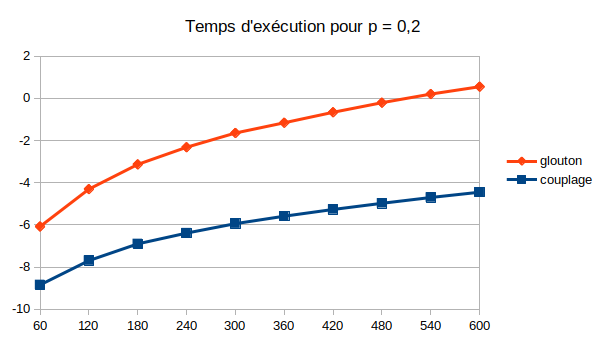
\includegraphics[scale=0.7]{figures/p2.png}
                    \centering
                \end{figure}

                \begin{figure}[h]
                    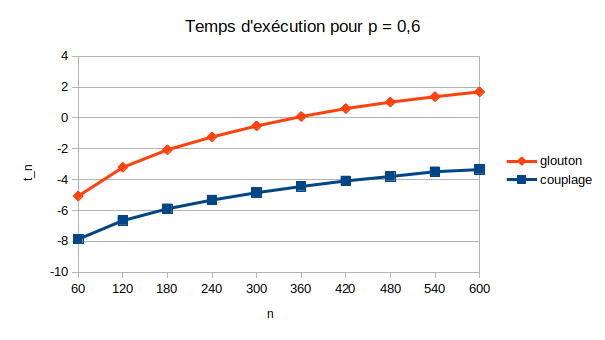
\includegraphics[scale=0.7]{figures/p6.png}
                    \centering
                \end{figure}

                \begin{figure}[h]
                    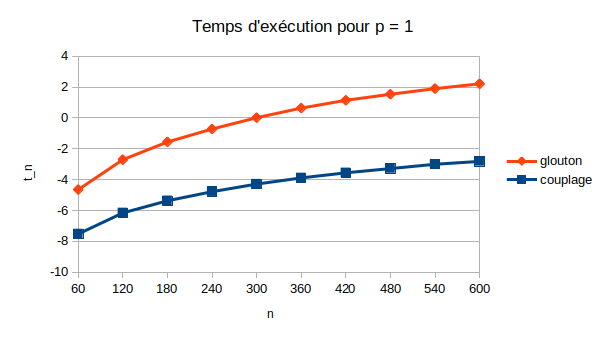
\includegraphics[scale=0.7]{figures/p10.png}
                    \centering
                \end{figure}
                
            De ces graphiques, nous pouvons observer que pour les deux algorithmes, le temps de calcul augmente de façon linéaire avec $n$ et $p$, et que algo\_glouton est nettement meilleur que algo\_couplage. \\
            Nous pouvions nous y attendre puisque algo\_couplage est en $O(nm)$ et algo\_glouton en $O(??)$

            \item \textit{Comparaison du point de vue de la qualité de la solution} :  
                %TODO

                Le facteur principal afin d'évaluer la qualité des solutions correspond à la dimension (longueur si on réflechit en fonction de structures de données) de la couverture.
                Nous allons donc analyser la dimension retournée par les methodes en rapport à la solution optimale.
                On va prendre la moyenne sur 3 essais sur 30 $N$ différents jusqu'à 600.

                \paragraph{$p = 1$} 
                Avec des graphes complets nous retrouvons des résultats très proches entre les deux méthodes, en effet le rapport est :
                $\dfrac{dim_{glouton}}{dim_{couplage}} = 0.993 $

                Nous sommes en dessus d'une différence de 5\%, donc on peut supposer de préferer dans ce cas la methode mieux approchée ou plus rapide, selon les nécessités.
                \begin{figure}[H]
                    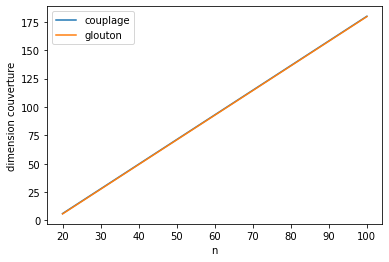
\includegraphics[scale=0.5]{figures/qualite_1.png}
                    \centering
                \end{figure}

                \paragraph{$p = 0.25$}{
                    Nous observons que même en réduisant $p$ jusqu'à $0.25$ (on a bien sûr effectué des test intérmediaires, que nous exclusons de cet document car il n'apportent pas des résultats hors de cette direction) les résultats ne varient beaucoup non plus.
                    
                    En effet, $\dfrac{dim_{glouton}}{dim_{couplage}} = 0.938 $ reste un rapport relativement petit.
                    
                    \begin{figure}[H]
                        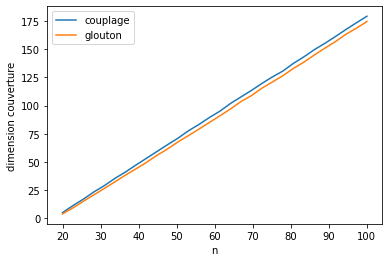
\includegraphics[scale=0.5]{figures/qualite_025.png}
                        \centering
                    \end{figure}
                }
                \paragraph{$p = 1/ \sqrt{n}$}
                    Ce n'est qu'avec des graphes particulièrement vides qu'on commence à observer une différence de qualité remarquable.

                    
                    En effet, $\dfrac{dim_{glouton}}{dim_{couplage}} = 0.858 $.
                    La méthode glouton prend le dessus dans ce cas de figure, cela nous indique que avec des graphes de plus en plus vides on s'approche aux cas limites de l'algorithme couplage.
                    \begin{figure}[H]
                        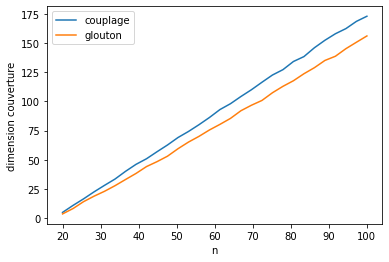
\includegraphics[scale=0.5]{figures/qualite_p.png}
                        \centering
                    \end{figure}


                Nous remarquons que le long de tous les essais, l'algorithme glouton est resté avec une écart inférieur de 5\% avec les solution optimales, alors que le couplage oscillait autour de 10-15\% selon les conditions.

                \begin{figure}[H]
                    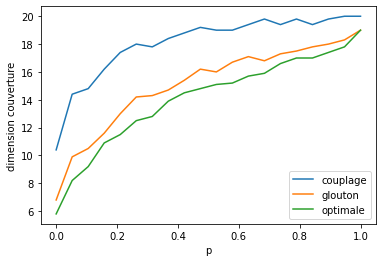
\includegraphics[scale=0.5]{figures/qualite_pvar.png}
                    \centering
                \end{figure}
                
                En moyenne, avec un graphe avec $n=20$ et en faisant varier p on a $\dfrac{dim_{glouton}}{dim_{optimale}} = 1.083 $ contre $\dfrac{dim_{couplage}}{dim_{optimale}} = 1.334 $.
                De plus, avec p qui varie de 0 à 1 on obtient le tableau suivant pour $\dfrac{dim_{glouton}}{dim_{couplage}}$ est :

                \begin{center}
                    \begin{tabular}{ |c c c c c| } 
                    \hline
                    0.65384615 & 0.6875 &    0.70945946  & 0.71604938 & 0.74712644  \\
                    0.78888889 & 0.80337079 & 0.79891304 & 0.81914894 & 0.84375   \\
                    0.84210526  & 0.87894737 & 0.8814433 & 0.84848485 & 0.89175258 \\
                     0.88383838 &  0.91752577 & 0.90909091 & 0.915   &    0.95\\
                    \hline
                    \end{tabular}
                    \end{center}


                Nous concludons affirmant que le choix de glouton se révele meilleur en terme de qualité malgré le temps d'execution plus grand.
                Avec des graphes complets la différence peut être considéré négligeable, mais avec des graphes 'vides' l'algorithme glouton prend un avantage plutôt fort.

        \end{enumerate}
        
    %\paragraph{3)}
        %Supposons qu'il existe $r$ tel que algo\_glouton soit $r$-approché.

\section{Méthodes exactes : algorithme de branch-and-bound}

    \paragraph{1.2)}
        Voici le tableau contenant le temps de calcul de la fonction branch en fonction de $n$.
        %TODO  

    \paragraph{2.1)}
        Soit $G=(V,E)$ un graphe non orienté, où $V$ est l'ensemble des sommets de et $E$ l'ensemble des arêtes. On note $n = |V|$ et $m = |E|$. \\
        Soit $M$ un couplage et $C$ une couverture de $G$. \\
        Posons $b_1 = \lceil \frac{m}{\Delta} \rceil$, $b_2 = |M|$ et $b_3 = \frac{2n-1 - \sqrt{(2n-1)^2 - 8m}}{2}$. \\
        Montrons que $|C| \geq b_1,b_2,b_3$.

        \begin{itemize}
            \item Soit $\Delta$ le degré maximum des sommets de $G$. Comme chaque sommet de $C$ est une extrémité d'au plus $\Delta$ arêtes, on a : $|C| \times \Delta \geq m \implies |C| \geq \frac{m}{\Delta}$. \\
            $|C|$ étant un entier, on peut prendre $b_2 = \lceil \frac{m}{\Delta} \rceil$ comme borne inférieure (???). 
            \item Pour toute arête de $M$, une de ses extrémités est dans $C$ (sinon elle ne serait pas couverte et $C$ ne serait pas une couverture). De plus, ces extrémités sont toutes distinctes par définition d'un couplage. Ainsi on a bien $\boxed{|C| \geq b_2}$
            \item ??? [ça ressemble à la formule d'une racine d'un polynôme du second degré.]
        \end{itemize}


\end{document}